\subsubsection{Analyse mit CMD}\label{A3.3.1}

\begin{figure}[H]
  \begin{center}
    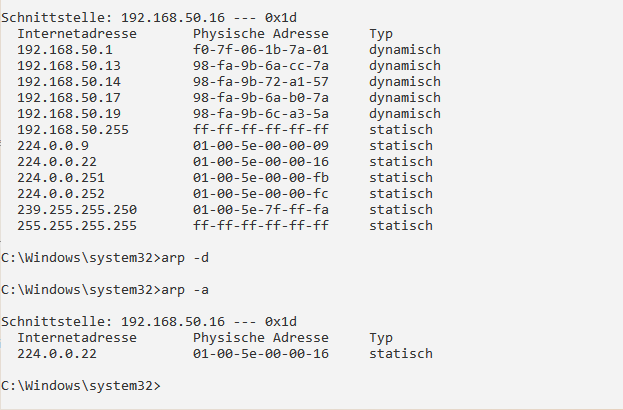
\includegraphics[width=0.618\textwidth]{graphics/versuch/3_3/arp_d}
    \caption{Löschen des ARP-Caches und folgendes Anzeigen der ARP-Tabelle}\label{abb_arp_d}
  \end{center}
\end{figure}

Im ersten Schritt wurde die ARP-Tabelle über die Eingabeaufforderung mithilfe von \inlinecode{arp -d} vollständig gelöscht (Abb. \ref{abb_arp_d}). Danach wurde der Nachbarrechner mit der IP-Adresse \inlinecode{192.168.50.14} mit dem \emph{ping}-Befehl angesprochen. Der Befehl hat den Zielrechner zuerst nach 4 Versuchen nicht erreicht, was daran lag, dass die Firewall am Ziel nicht deaktiviert war und den ping nicht durchgelassen hat. Nach Deaktivierung der Firewall lieferte der Befehl erfolgreiche Ergebnisse (Abb. \ref{abb_ping_1}).


\begin{figure}[H]
  \begin{center}
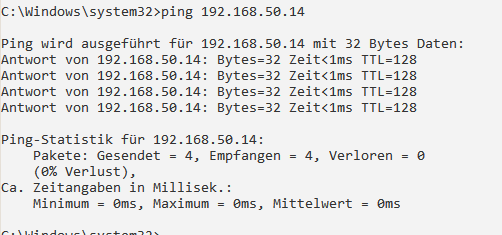
\includegraphics[width=0.618\textwidth]{graphics/versuch/3_3/ping_nach_abschalten_firewall_auf_zielrechner}
    \caption{Ping des Nachbarrechners 192.168.50.14}\label{abb_ping_1}
  \end{center}
\end{figure}

Nach dem ping-Befehl wurde erneut die ARP-Tabelle angezeigt (Abb \ref{abb_arp_neu}). Man kann erkennen, dass die IP-Adresse des Nachbarrechners in den Cache aufgenommen wurde. Außerdem wurde auch eine andere Adresse als Resultat des Empfangs einer ping-Nachricht aufgenommen, nämlich die \inlinecode{192.168.50.17}.

\begin{figure}[H]
  \begin{center}
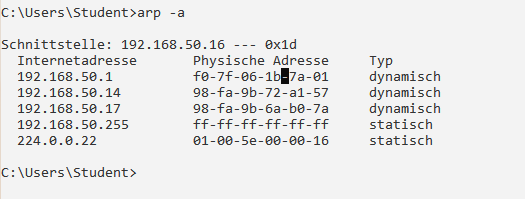
\includegraphics[width=0.618\textwidth]{graphics/versuch/3_3/arp_a_nach_ping_von_nachbar}
    \caption{ARP-Tabelleneinträge nach Ausführen des ping-Befehls}\label{abb_arp_neu}
  \end{center}
\end{figure}

Da der ping-Befehl, wie auch alle anderen Daten, durch Schicht 1 und 2 läuft, benötigt er die MAC-Adressen des Ziels, muss also die angegebene IP-Adresse übersetzen. Da die ARP-Tabelle gelöscht wurde, kann diese nicht zum Nachschlagen verwendet werden, weshalb ein ARP-Broadcast an alle Teilnehmer des Netzwerkes gesendet werden muss, um anzufragen, welche MAC-Adresse zum Host \inlinecode{192.168.50.14} gehört. Die notwendige Broadcast-Adresse ist wie in \ref{A3.2.2} ermittelbar, daher erscheint sie auch in Abb. \ref{abb_arp_neu}.\\

Die Multicast-Adresse \inlinecode{224.0.0.22} scheint fest eingebaut zu sein, da diese bereits in Abb. \ref{abb_arp_d} unmittelbar nach dem Löschen des ARP-Caches zu sehen war.

\subsubsection{Analyse mit Wireshark}
Mithilfe des Filters \inlinecode{arp || icmp} können nur die Pakete der für die Auswertung relevanten Protokolle betrachtet werden.\\


\begin{figure}[H]
  \begin{center}
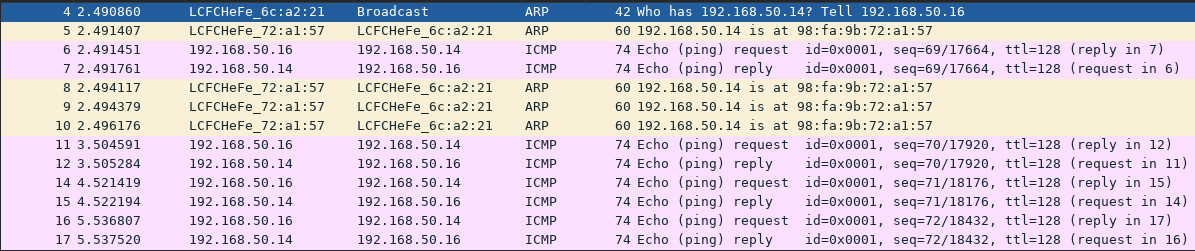
\includegraphics[width=\textwidth]{graphics/versuch/3_3/wireshark/allgemein}
    \caption{Gefilterte Ausgabe von Wireshark bei senden des ping-Kommandos}\label{wire_ping}
  \end{center}
\end{figure}

\paragraph{ARP}\label{A2.3.2.arp}
In Abb. \ref{wire_ping} erkennt man ersteinmal, dass genau 8 ICMP-Pakete aufgezeichnet wurden. Davon sind 4 Anfragen und 4 Antworten. Dies deckt sich mit Abb. \ref{abb_ping_1}, da der ping-Befehl genau 4 Mal gesendet wurde.\\

Vor Beginn des eigentlichen Pings findet man ein ARP-Paket. Hierbei handelt es sich um eine Broadcast-Nachricht zum Bestimmen der MAC-Adresse des Ziels. Dies ist notwendig, da vorher der ARP-Cache gelöscht wurde und sich dort kein Eintrag zur Ziel-IP-Adresse befindet (vgl. \ref{A3.3.1}).\\

Betachtet man die ARP-Anfrage genauer (Abb. \ref{arp_broadcast}), erkennt man im Ethernet-Frame, dass die Ziel-MAC-Adresse die bereits genannte \inlinecode{ff:ff:ff:ff:ff:ff} ist, welche für den Broadcast reserviert ist. Aus dem Quell-Feld erkennt man nun auch die Adresse der eigenen Netzwerkschnittstelle, nämlich \inlinecode{98:fa:9b:6c:a2:21}. Weiterhin ist im Header, wie zu erwarten, der Ethertype ARP, angegeben.

\begin{figure}[H]
  \begin{center}
    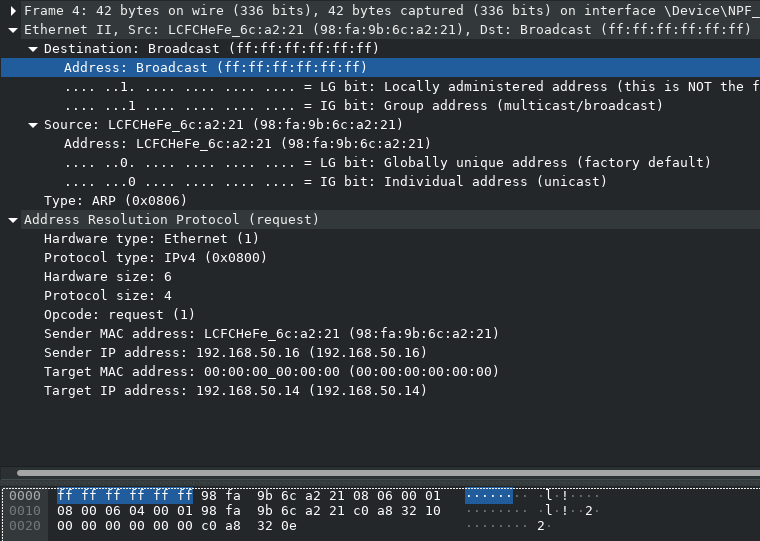
\includegraphics[width=\textwidth]{graphics/versuch/3_3/wireshark/arp_broadcast}
    \caption{Genauere Analyse der ersten ARP-Anfrage}\label{arp_broadcast}
  \end{center}
\end{figure}

Im folgenden Nutzdatenfeld befindet sich die ARP-Anfrage. Hier steht der Opcode 1 um zu signalisieren, dass es sich um eine Anfrage handelt. Außerdem enthält es Sender-MAC und -IP Adressen, sowie die bekannte Ziel-IP-Adresse. Das Feld Ziel-MAC-Adresse ist frei, da genau diese ja nachgefragt werden soll. Der angesprochene Host (sofern existent) sollte antworten und beide Felder ausfüllen. Dies geschieht dann auch in der zweiten Zeile von Abb. \ref{wire_ping}, in welcher die ARP-Antwort empfangen wurde.\\

Es antwortet also genau der Host auf den Broadcast mit einer ARP-Nachricht, dem die angefragte MAC-Adresse gehört. In Abb. \ref{arp_answer} ist der genaue Inhalt der ARP-Anwort dargestellt. Die Ziel-MAC ist nun nicht mehr der Broadcast, sondern die Adresse des Anfragers, die aus der Anfrage entnommen werden konnte. Mit dem Empfang dieser Daten ist das Ziel des ping-Befehls identifiziert.

\begin{figure}[H]
  \begin{center}
    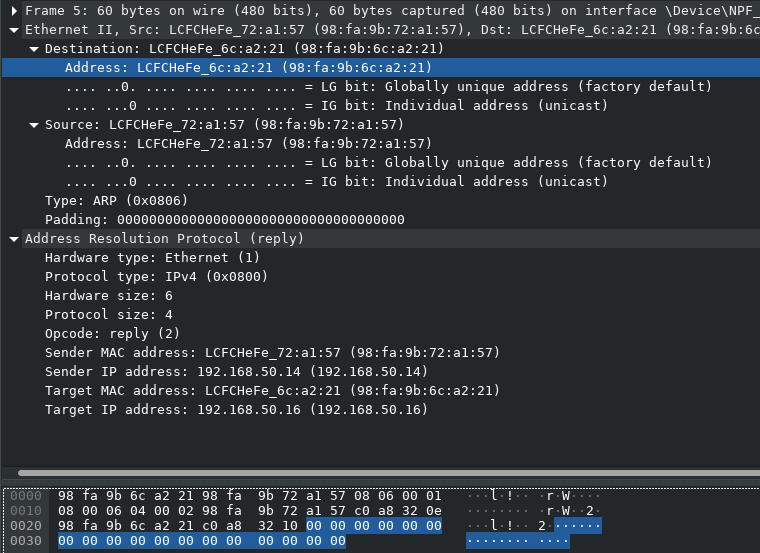
\includegraphics[width=\textwidth]{graphics/versuch/3_3/wireshark/arp_answer}
    \caption{Antwort auf die ARP-Anfrage}\label{arp_answer}
  \end{center}
\end{figure}

\label{CRC_erklar} Auffällig ist, dass in der Antwort aus Abb. \ref{arp_answer} im Ethernetframe zusätzlich ein 18-Byte langes Padding-Feld aus Nullen hinzugefügt wurde. Dies wird benötigt, um die minimale Länge des Frames von $64$ Byte zu erreichen. In Wireshark sind jedoch nur 60 Byte angezeigt, was daran liegt, dass das 4 Byte lange FCS-Feld zur Fehlererkennung mittels CRC automatisch weggelassen wird.\\

Dass die Framegröße in Abb. \ref{arp_broadcast} nur 42 und nicht 60 Byte lang ist, liegt daran, dass es sich um ein Paket handelt, das von der Schnittstelle gesendet wurde, die auch aufgezeichnet wird. In diesem Fall werden die Daten aufgezeichnet, bevor das Padding angefügt wird.\\

\paragraph{ICMP}
Da der ping-Befehl das ICMP-Protokoll verwendet, findet man dieses auch im Wireshark-Trace wieder, z.B. bei der ersten Anfrage (Abb. \ref{icmp_request}). Die allgemeine Struktur eines ICMP-Paketes ist in Abb. \ref{icmp_header} zu sehen.


\begin{figure}[H]
\centering
\resizebox{0.618\textwidth}{!}{\import{graphics/}{icmp_header.pdf_tex}}
\caption{Struktur des ICMP-Paketes}\label{icmp_header}
\end{figure}

Das Typ-Feld kann Werte von 0-255 annehmen und gibt die Art der Kontrollnachricht\footnote{\url{wikipedia.org/Internet_Control_Message_Protocol}} an. Beispielsweise bedeutet der Typ-Wert 0 eine Echo-Reply Nachricht (Echo Antwort, verwendet von ping) und der Wert 8 ein Echo-Request (Echo-Anfrage). Das Code-Feld gibt hierbei zusätzliche Informationen zum jeweiligen Typ-Feld. Bei den ICMP-Typen des ping-Befehls, also Echo-Reply und -Request ist der Inhalt des Code-Feldes 0.

\begin{figure}[H]
  \begin{center}
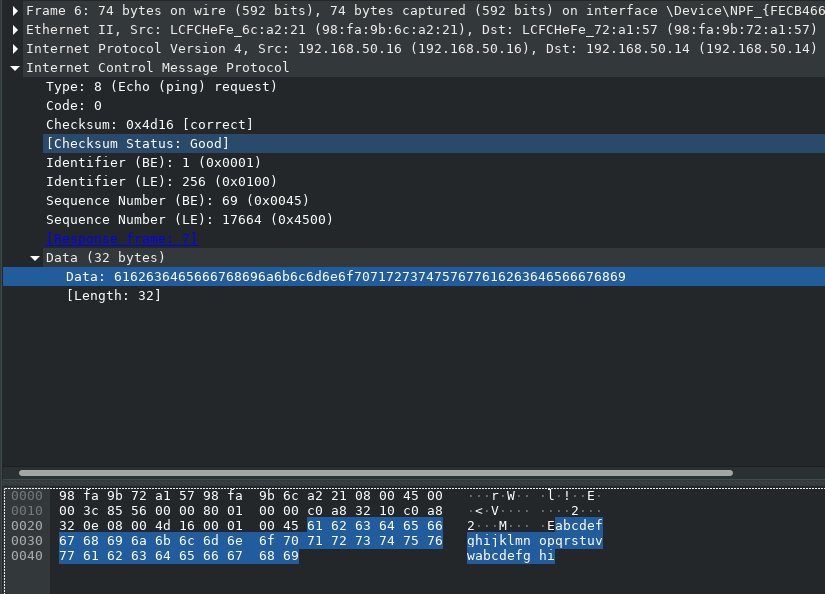
\includegraphics[width=\textwidth]{graphics/versuch/3_3/wireshark/ping_request}
    \caption{ICMP-Anfrage des ping-Befehls, Ausgabe von Wireshark mit geöffnetem ICMP-Paket}\label{icmp_request}
  \end{center}
\end{figure}

Auffällig ist hierbei zuerst, dass, im Gegensatz zum ARP-Beispiel, die ICMP-Daten in ein IP-Paket gepackt sind (Zeile 3 in Abb. \ref{icmp_request}). Das ist auch sinnvoll, da ICMP auf Ebene 3 agiert und eine konkrete Ziel-IP-Adresse benötigt, während ARP auf Ebene 2 mithilfe von Broadcasts arbeitet und somit nicht in Berührung mit dem IP-Header kommt.\\

Das ICMP-Paket in diesem Beispiel hat ein 32 Byte langes Datenfeld (max. ), welches mit 32 diversen ASCII-Zeichen gefüllt ist. Die Ausgabe der Eingabeaufforderung in Abb. \ref{abb_ping_1} bestätigt dies. Die Gesamtgröße des Paketes ist 40 Byte (abzählbar aus Wireshark-Ausgabe), die Header-Größe ist daher die Differenz, also 8 Byte, was auch mit der ICMP-Definition übereinstimmt.\\

Folgend kommt die ICMP-Antwort, wie sie in Abb. \ref{icmp_answer} zu sehen ist, vom erwarteten Host mit der  IP-Adresse \inlinecode{192.168.50.14}. Die Antwort enthält die gleichen Zeichen im ICMP-Datenfeld, nur das Typ-Feld wurde geändert von 8 (request) auf 0 (reply), was ebenfalls zu erwarten war.

\begin{figure}[H]
  \begin{center}
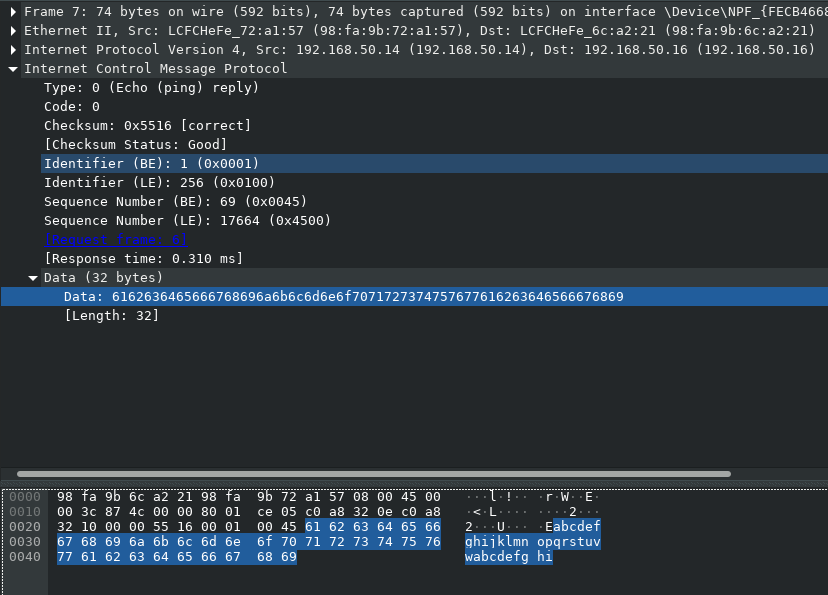
\includegraphics[width=\textwidth]{graphics/versuch/3_3/wireshark/ping_answer}
    \caption{ICMP-Antwort auf die Anfrage durch den ping-Befehl}\label{icmp_answer}
  \end{center}
\end{figure}

Der gesamte Ping-Prozess wird, wie bereits erwähnt, vier Mal wiederholt. Die dabei gesendeten bzw. empfangenen Pakete/Frames sind einschließlich des Datenfeldes äquivalent zu denen des ersten Pings, der hier behandelt wurde (nur Quell/Ziel-Adressen sind vertauscht).\\

Die Zeiten, die die CMD-Ausgabe des Befehls angibt, können ebenfalls in Wireshark bestätigt werden. In Abb. \ref{abb_ping_1} wird eine Zeit $<1\,\si{\milli\second}$ berichtet. Aus der Zeitdifferenz in Wireshark ergeben sich $310 \,\si{\micro\second}$.\\

In Abb. \ref{wire_ping} erkennt man 3 weitere ARP-Antworten vom Host \inlinecode{192.168.50.14}, obwohl nur eine Anfrage gestellt wurde. Die Antworten sind der bereits empfangenen ersten Antwort identisch. Weshalb genau diese erscheinen, konnte nicht geklärt werden.\\

\subsubsection{Flussdiagramm der Ping-Kommunikation}


\begin{figure}[H]
\centering
    \resizebox{\textwidth}{!}{\import{graphics/}{ping_flowchart.pdf_tex}}
    \caption{Flussdiagramm der Ping-Kommunikation}
\end{figure}

Das Flussdiagramm stellt den zeitlichen Ablauf der Kommunikation zwischen Sender (\inlinecode{192.168.50.16}) und Empfänger (\inlinecode{192.168.50.16}) dar. Für Sender und Empfänger sind jeweils die IP-Adressen als Endpunkt angegeben, allerdings sind diese nur für das Verständis, da nicht jedes Protokoll (wie z.B. ARP) diese zur Adressierung benötigt. Die Zeitangaben sind jeweils als sogenannte \glqq Delta Zeit\grqq, also der Zeitdifferenz zum vorherigen Ereignis dargestellt (Laufzeit, Wireshark $\rightarrow$ Einstellungen $\rightarrow$ Columns $\rightarrow$ delta Time).\\

Der Einfachheit halber wurden im Flussdiagramm nicht alle Felder der jeweiligen Pakete, sondern nur die für das Verständis der Kommunikation notwendigen dargestellt.

\subsubsection{ping-Overhead}
Für die Betrachtung des prozentualen Overheads wird das gesamte ICMP-Paket, so wie es der IP-Header umfasst, betrachtet. Wie vorher bereits bestimmt, beträgt die Größe dieses Paketes $32 \, \si{\byte} + 8 \, \si{\byte} = 40$ Byte. Der gesamte Frame, so wie er in das Netzwerk übertragen wird, beträgt laut Wireshark $74 \, \si{\byte}$ zu denen noch $4 \, \si{\byte}$ für das Ethernet-FCS Feld hinzukommen (siehe \ref{CRC_erklar}/ARP). Somit sind es $74 + 4 - 32 = 46$ Byte an Overhead. Der Prozentuale Overhead $o$ des ping-Befehls (genauer: des Standard-ping-Befehls unter Windows) ist demnach
\[o = \frac{46 \, \si{\byte}}{78 \, \si{\byte}} \cdot 100 \, \si{\percent} \approx 59 \, \si{\percent}\,.\]
